\documentclass[9pt]{beamer}
% \documentclass[notes, handout, 9pt]{beamer}
% \documentclass[handout, 9pt]{beamer}

\usepackage{import}
\subimport{../}{preamble.tex}
\subimport{../}{beamer-theme.tex}
\usepackage{svg}

% Location for all figures / pictures
\graphicspath{{pictures/}{figures/}}

% % Figures inline
\usepackage{tikz}
\usepackage{pgfplots}
\usetikzlibrary{calc}
\usetikzlibrary{positioning}
\usetikzlibrary{shapes.multipart}
\usetikzlibrary{decorations.pathreplacing}
\usetikzlibrary{arrows.meta}
\usepgfplotslibrary{fillbetween}
\pgfplotsset{compat=1.16}

% Hadamard product shorthand
\newcommand{\had}{\odot}

%--------------------------------------------------
% Presentation Information
%--------------------------------------------------
\title[Continuous Optimization]{Neural Networks and Automatic Differentiation}
\author[]{\textbf{Bart Van Parys}}
\date[]{Fall 2026}
%--------------------------------------------------

\begin{document}

\begin{frame}

  \maketitle

  \vspace{-2em}

    \begin{center}
    \begin{tabular}{lll}
      Instructor : & \textbf{Bart Van Parys} & \textbf{(\href{mailto:mastermath@vanparys.xyz}{mastermath@vanparys.xyz})} \\
    \end{tabular}
  \end{center}

\end{frame}

\begin{frame}{Where we are}

  Today we turn to the ``killer app'' of black box optimization : \emph{deep learning}.
  The problems are
  \begin{itemize}
    \setlength\itemsep{0.5em}
  \item \emph{enormous} --- millions to billions of variables,
  \item \emph{non-convex} --- none of our global guarantees apply,
  \item and yet \emph{solved routinely} by the simplest tool we own: SGD.
  \end{itemize}

\end{frame}

\begin{frame}{Why the excitement? A 2026 headline}

  \begin{columns}[T]
    \begin{column}{0.56\textwidth}
      A classical question of Erd\H{o}s (1946): among $n$ points in the plane,
      how many pairs can be at \emph{exactly} unit distance?

      \medskip

      \textbf{Def}:
        \[
          u(n) \defn \max_{\substack{P\subseteq\Re^2,\ |P|=n}}
          \,\bigl|\{\,\{p,q\}\subseteq P : \norm{p-q}=1\,\}\bigr|,
        \]
        the largest number of \emph{unordered} unit-distance pairs over all
        $n$-point sets.
     
    \end{column}

    \begin{column}{0.42\textwidth}
      \begin{center}
        \includesvg[width=0.80\textwidth]{pictures/unit-distance.svg}\\[0.2em]
        {\scriptsize $16$ points, $40$ unit distances.}
      \end{center}
    \end{column}
  \end{columns}

  \medskip
  
  \uncover<2->{
    Erd\H{o}s \emph{conjectured} : $u(n) = n^{1+o(1)}$.
  }
  
  \medskip

  \uncover<3->{
  \textbf{Thm:} (OpenAI 2026) There is a $\delta \geq 0.014$ with $u(n) \geq n^{\,1+\delta}$ for infinitely many $n$.
  }

\end{frame}


\section{Neural Networks: What and Why}


\begin{frame}{Empirical Risk Minimization --- a reminder}

  Recall from the previous lecture the \emph{empirical risk minimization} problem
  \[
    \min_{x\in\Re^n} ~f(x) \defn \frac{1}{T} \sum_{i=1}^T \ell(h_x(\omega_i), y_i)
  \]
  where $(\omega_i, y_i)$ are data points, $\ell$ a loss, and $h_x$ a \emph{model}
  parametrised by $x\in\Re^n$.

  \vfill

  \uncover<2->{
  \begin{itemize}
    \setlength\itemsep{0.6em}
  \item Linear regression (Lecture 1): $h_x(\omega) = \iprod{x}{\omega}$ and $\ell(\hat y_i, y_i)=\norm{y_i-y_i}^2_2$. \quad \green{Convex.}
  \item<3-> \emph{Neural network}: $h_x$ a composition of affine maps and
    nonlinearities. \quad \red{Non-convex.}
  \end{itemize}
  }

\end{frame}

\begin{frame}{What is a neural network?}

  A \emph{feed-forward network} with $L$ layers maps an input
  $a^0 = \omega \in \Re^{d_0}$ to an output $h_x(\omega) = a^L$ through the recursion
  \begin{align*}
    z^l &= W^l a^{l-1} + b^l, \qquad &&\text{(affine / pre-activation)}\\
    a^l &= \sigma(z^l),       \qquad &&\text{(fixed nonlinearity)}
  \end{align*}
  for $l = 1, \dots, L$. The parameters are $x = (W^1, b^1, \dots, W^L, b^L)$ with
  $W^l\in\Re^{d_l\times d_{l-1}}$.

  \vfill

  \begin{center}
    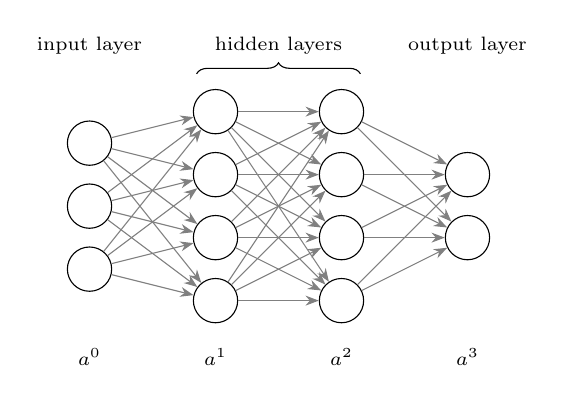
\begin{tikzpicture}[
      x=1.6cm, y=0.8cm, >=Stealth,
      neuron/.style={circle, draw, minimum size=16pt, inner sep=0pt},
      every node/.style={font=\scriptsize}]

      \foreach \l/\n/\lab in {0/3/{$a^0$}, 1/4/{$a^1$}, 2/4/{$a^2$}, 3/2/{$a^3$}}{
        \foreach \i in {1,...,\n}{
          \node[neuron] (N\l\i) at (\l, {(\n-1)/2 - (\i-1)}) {};
        }
        \node at (\l, -2.4) {\lab};
      }
      % edges
      \foreach \a in {1,2,3}{ \foreach \b in {1,2,3,4}{ \draw[->, gray] (N0\a) -- (N1\b);}}
      \foreach \a in {1,2,3,4}{ \foreach \b in {1,2,3,4}{ \draw[->, gray] (N1\a) -- (N2\b);}}
      \foreach \a in {1,2,3,4}{ \foreach \b in {1,2}{ \draw[->, gray] (N2\a) -- (N3\b);}}
      % layer labels
      \node at (0, 2.55) {input layer};
      \node at (1.5, 2.55) {hidden layers};
      \node at (3, 2.55) {output layer};
      \draw[decorate, decoration={brace, amplitude=4pt}]
        (0.85, 2.1) -- (2.15, 2.1);
    \end{tikzpicture}
  \end{center}

\end{frame}

\begin{frame}{Activation functions}

  The nonlinearity $\sigma$ is what makes the model more than one big affine map.

  \vfill

  \begin{columns}[T]
    \begin{column}{0.33\textwidth}
      \centering
      \begin{tikzpicture}
        \begin{axis}[width=4.4cm, height=3.4cm, title={sigmoid $\tfrac{1}{(1+e^{-z})}$},
          title style={font=\scriptsize}, axis lines=middle, ticks=none,
          xmin=-3, xmax=3, ymin=-0.25, ymax=1.25, domain=-3:3, samples=80]
          \addplot[blue, thick] {1/(1+exp(-3*x))};
        \end{axis}
      \end{tikzpicture}
    \end{column}
    \begin{column}{0.33\textwidth}
      \centering
      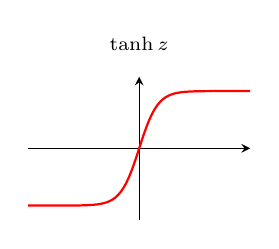
\begin{tikzpicture}
        \begin{axis}[width=4.4cm, height=3.4cm, title={$\tanh z$},
          title style={font=\scriptsize}, axis lines=middle, ticks=none,
          xmin=-3, xmax=3, ymin=-1.25, ymax=1.25, domain=-3:3, samples=80]
          \addplot[red, thick] {tanh(2*x)};
        \end{axis}
      \end{tikzpicture}
    \end{column}
    \begin{column}{0.33\textwidth}
      \centering
      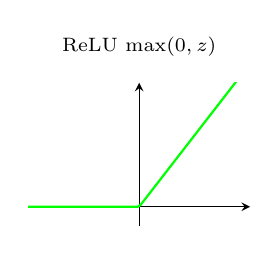
\begin{tikzpicture}
        \begin{axis}[width=4.4cm, height=3.4cm, title={ReLU $\max(0,z)$},
          title style={font=\scriptsize}, axis lines=middle, ticks=none,
          xmin=-3, xmax=3, ymin=-0.4, ymax=2.6, domain=-3:3, samples=80]
          \addplot[green, thick] {max(0,x)};
        \end{axis}
      \end{tikzpicture}
    \end{column}
  \end{columns}

  \vfill

  \begin{itemize}
    \setlength\itemsep{0.4em}
  \item \emph{Sigmoid / tanh}: smooth, but saturate --- gradients vanish for large $|z|$.
  \item<2-> \emph{ReLU}: piecewise linear, cheap, non-saturating; the modern default.
    Non-differentiable only at the single point $z=0$.
  \end{itemize}

\end{frame}

\begin{frame}{Why a nonlinearity at all?}
  
  \textbf{Universal Approximation (Cybenko 1989, Hornik 1991):} a network with one
  hidden layer and a non-polynomial activation can approximate \emph{any} continuous
  function on a compact set to arbitrary accuracy, given enough width.

  \vfill

  \uncover<2->{
  \begin{itemize}
  \item Expressivity is \emph{not} the issue --- even shallow nets are universal.
  \item The real questions are \emph{optimization} (can we fit it?) and
    \emph{generalization} (does the fit transfer?).
  \end{itemize}
  }

\end{frame}

\begin{frame}{A very short history}

  \begin{center}
  \begin{tabular}{r@{\quad}l}
    \hline
    \textbf{1943} & McCulloch \& Pitts: a mathematical model of a neuron.\\[0.3em]
    \textbf{1958} & Rosenblatt: the \emph{perceptron} --- learning from data.\\[0.3em]
    \textbf{1969} & Minsky \& Papert: perceptrons cannot learn \texttt{XOR}. \red{First AI winter.}\\[0.3em]
    \textbf{1986} & Rumelhart, Hinton \& Williams: \emph{backpropagation} popularised.\\[0.3em]
    \textbf{1989} & LeCun: convolutional nets read handwritten digits.\\[0.3em]
    \textbf{1998--2010} & Kernel methods \& SVMs dominate; nets out of fashion.\\[0.3em]
    \textbf{2012} & \emph{AlexNet} wins ImageNet by a landslide. \green{Deep learning era begins.}\\[0.3em]
    \textbf{2014} & \blue{Kingma} \& Ba: the \emph{Adam} optimiser (\textsection 3 today). Kingma \& Welling: VAEs.\\[0.3em]
    \textbf{2017} & \emph{Transformers}: ``attention is all you need''.\\[0.3em]
    \textbf{2020--} & Large language models; scaling laws; generative AI.\\[0.3em]
    \hline
  \end{tabular}
  \end{center}

  \vfill

  \uncover<2->{
  The \emph{ideas} are old. What changed is \emph{why they work now}.
  }

    \medskip
    \uncover<3->{
      {\footnotesize \blue{A Dutch thread:} the \emph{Adam} optimiser of \textsection 3 is due to \textbf{Diederik Kingma} --- undergrad at \emph{Utrecht}, PhD at the \emph{University of  Amsterdam} with Max Welling. And the language it all runs on, \emph{Python}, was created by \textbf{Guido van Rossum} at \emph{CWI} in Amsterdam. }
  }

\end{frame}

\begin{frame}{Why now? Three ingredients}

  \begin{columns}[t]
    \begin{column}{0.32\textwidth}
      
      \centering
      \begin{minipage}[c][1.85cm][c]{\linewidth}
        \centering
        % database cylinder
        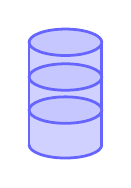
\begin{tikzpicture}[scale=0.42, line join=round]
          % body incl. bottom cap, as one closed (filled) path
          \fill[blue!18] (-1.1,1.55) -- (-1.1,-1.55) arc (180:360:1.1 and 0.4)
            -- (1.1,1.55) -- cycle;
          % vertical sides
          \draw[blue!60, line width=1pt] (-1.1,1.55) -- (-1.1,-1.55);
          \draw[blue!60, line width=1pt] (1.1,1.55) -- (1.1,-1.55);
          % front bottom curve
          \draw[blue!60, line width=1pt] (-1.1,-1.55) arc (180:360:1.1 and 0.4);
          % stacked disk tops (bottom to top)
          \foreach \y in {-0.5, 0.5, 1.55}{
            \draw[blue!60, fill=blue!22, line width=1pt] (0,\y) ellipse (1.1 and 0.4);
          }
        \end{tikzpicture}
      \end{minipage}
      \par\vspace{0.3em}
      \raggedright
      \textbf{\blue{Data}}
      \begin{itemize}
      \item Internet-scale labelled and unlabelled corpora.
      \item ImageNet ($14$M images), web text ($10^{12}$ tokens).
      \end{itemize}
      \vspace{0.8em}
      \begin{center}
\includegraphics[width=0.7\textwidth]{imagenet_logo.png}\end{center}
    \end{column}
    \begin{column}{0.32\textwidth}
      \uncover<2->{
      \centering
      \begin{minipage}[c][1.85cm][c]{\linewidth}
        \centering
        % graphics card PCB + shroud
        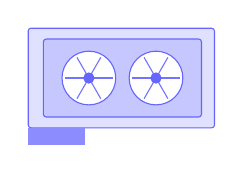
\begin{tikzpicture}[scale=0.55, line join=round]
          \fill[blue!12, draw=blue!60, rounded corners=1pt] (-0.2,-0.1) rectangle (4.1,2.2);
          \fill[blue!22, draw=blue!60, rounded corners=1pt] (0.15,0.15) rectangle (3.8,1.95);
          \foreach \cx in {1.2, 2.75}{
            \fill[white, draw=blue!60] (\cx,1.05) circle (0.62);
            \foreach \a in {0,60,...,300}{ \draw[blue!55] (\cx,1.05) -- ++(\a:0.55);}
            \fill[blue!60] (\cx,1.05) circle (0.13);
          }
          \fill[blue!45] (-0.2,-0.5) rectangle (1.1,-0.1);
        \end{tikzpicture}
      \end{minipage}
      \par\vspace{0.3em}
      \raggedright
      \textbf{\blue{Compute}}
      \begin{itemize}
      \item GPUs / TPUs: cheap parallel linear algebra.
      \item Training FLOPs doubling every few months.
      \end{itemize}
      }
    \end{column}
    \begin{column}{0.32\textwidth}
      \uncover<3->{
      \centering
      \begin{minipage}[c][1.85cm][c]{\linewidth}
        \centering
        % processor chip
        
\begin{tikzpicture}[scale=0.42, line join=round]
          \foreach \i in {0.5,1.0,...,2.4}{
            \draw[blue!55, line width=1pt] (\i,2.8)--(\i,3.2);
            \draw[blue!55, line width=1pt] (\i,0)--(\i,-0.4);
            \draw[blue!55, line width=1pt] (0,\i)--(-0.4,\i);
            \draw[blue!55, line width=1pt] (2.8,\i)--(3.2,\i);
          }
          \fill[blue!20, draw=blue!60, rounded corners=1.5pt, line width=1pt] (0,0) rectangle (2.8,2.8);
          \draw[blue!60, line width=1pt, rounded corners=1pt] (0.7,0.7) rectangle (2.1,2.1);
          \node[font=\scriptsize\bfseries, text=blue!70] at (1.4,1.4) {CPU};
        \end{tikzpicture}
      \end{minipage}
      \par\vspace{0.3em}
      \raggedright
      \textbf{\blue{Algorithms}}
      \begin{itemize}
      \item \emph{Automatic differentiation}: gradients for free.
      \item \emph{SGD / Adam}: scale to billions of parameters.
      \item ReLU, normalisation, residual connections.
      \end{itemize}
      }
    \end{column}
  \end{columns}

 
\end{frame}

\begin{frame}{The optimization problem we actually face}

  \begin{center}
    \begin{tabular}{r|l}
      \hline
      Optimization Problem & Neural network training \\[0.5em]
      \hline
      Model $\Sigma$ & $\min_{x\in \Re^n} f(x)=\tfrac{1}{T}\sum_{i=1}^T \ell(h_x(\omega_i), y_i)$ \\[0.5em]
                     & $f$ is \red{non-convex}, $L$-smooth (typically), $n$ huge\\[0.5em]
      Oracle $\mc O$ & stochastic first-order oracle $x\mapsto \hat f'(x)$\\[0.5em]
      Accuracy $\mc T_\epsilon$ & find $\hat x$ with small \emph{test} loss (not just training!)\\[0.5em]
      \hline
    \end{tabular}
  \end{center}

  \vfill

  \textbf{What our theory does \emph{not} give us:}
  \begin{itemize}
    \setlength\itemsep{0.4em}
  \item No global minimum guarantee --- SGD finds a \emph{stationary point}, at best.
  \item<2-> No reason a low \emph{training} loss implies a low \emph{test} loss.
  \end{itemize}

  \vfill

  \uncover<3->{
  \emph{Remarkably}, in practice both work out. Understanding \emph{why} is the
  frontier --- and the subject of the last part of this lecture.
  }

\end{frame}

\section{Automatic Differentiation}

\begin{frame}{The forward pass}

   \begin{center}
    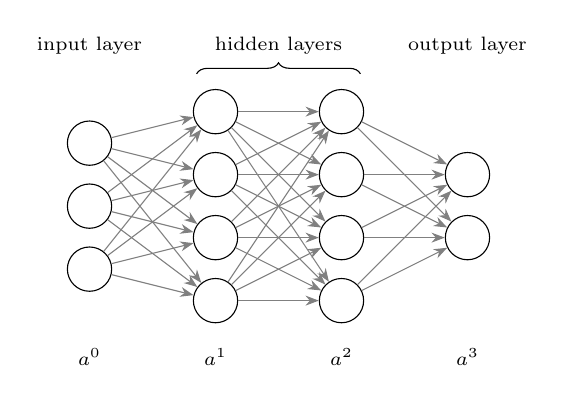
\begin{tikzpicture}[
      x=1.6cm, y=0.8cm, >=Stealth,
      neuron/.style={circle, draw, minimum size=16pt, inner sep=0pt},
      every node/.style={font=\scriptsize}]

      \foreach \l/\n/\lab in {0/3/{$a^0$}, 1/4/{$a^1$}, 2/4/{$a^2$}, 3/2/{$a^3$}}{
        \foreach \i in {1,...,\n}{
          \node[neuron] (N\l\i) at (\l, {(\n-1)/2 - (\i-1)}) {};
        }
        \node at (\l, -2.4) {\lab};
      }
      % edges
      \foreach \a in {1,2,3}{ \foreach \b in {1,2,3,4}{ \draw[->, gray] (N0\a) -- (N1\b);}}
      \foreach \a in {1,2,3,4}{ \foreach \b in {1,2,3,4}{ \draw[->, gray] (N1\a) -- (N2\b);}}
      \foreach \a in {1,2,3,4}{ \foreach \b in {1,2}{ \draw[->, gray] (N2\a) -- (N3\b);}}
      % layer labels
      \node at (0, 2.55) {input layer};
      \node at (1.5, 2.55) {hidden layers};
      \node at (3, 2.55) {output layer};
      \draw[decorate, decoration={brace, amplitude=4pt}]
        (0.85, 2.1) -- (2.15, 2.1);
    \end{tikzpicture}
  \end{center}

  \vfill

  \begin{itemize}
    \setlength\itemsep{0.5em}
  \item Its cost is dominated by the matrix products $W^l a^{l-1}$.
  \item This is the \emph{natural unit}: GPUs are built to run it, and everything else (loss, gradient) costs a small
    \emph{multiple of one forward pass}.
  \end{itemize}

\end{frame}

\begin{frame}{The gradient is everything}

  Every method in this course (gradient descent, Newton, SGD, Adam) needs
  $f'(x)$. For a network with $n=10^6$--$10^{12}$ parameters, \emph{how} do we get it?

  \vfill

  \begin{center}
    \begin{tabular}{l|l|l}
      \hline
      Approach & Idea & Verdict \\[0.4em]
      \hline
      \emph{Numerical} & $\partial_i f \approx \tfrac{(f(x+he_i)-f(x))}{h}$ & \red{$\mc O(n)$ passes, round-off}\\[0.4em]
      \emph{Symbolic} & differentiate the formula & \red{expression swell}\\[0.4em]
      \emph{Automatic} & chain rule on the \emph{computational graph} & \green{exact, $\mc O(1)$ passes}\\[0.4em]
      \hline
    \end{tabular}
  \end{center}

  \vfill

  \uncover<2->{
  \emph{Automatic differentiation} (AD) is neither numerical nor symbolic: it applies
  the chain rule \emph{numerically}, step by step, to the program that computes $f$.
  }

\end{frame}

\begin{frame}{The computational graph}

  Any function built from elementary operations is a directed acyclic graph. Take
  \[
    f(x_1,x_2) = x_1 x_2 + \sin(x_1).
  \]

  \vfill

  \begin{center}
    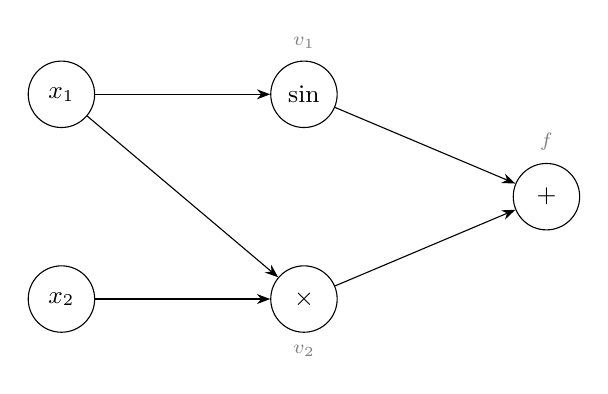
\begin{tikzpicture}[
      x=2.2cm, y=1.3cm, >=Stealth,
      vtx/.style={circle, draw, minimum size=24pt, inner sep=1pt, font=\small},
      vlab/.style={font=\scriptsize, gray}]
      % each operation lives INSIDE its node; edges are plain data flow
      \node[vtx] (x1) at (0,1)  {$x_1$};
      \node[vtx] (x2) at (0,-1) {$x_2$};
      \node[vtx] (v1) at (1.4,1)  {$\sin$};
      \node[vtx] (v2) at (1.4,-1) {$\times$};
      \node[vtx] (f)  at (2.8,0)  {$+$};
      % name each intermediate node by the value it produces
      \node[vlab, above=1pt of v1] {$v_1$};
      \node[vlab, below=1pt of v2] {$v_2$};
      \node[vlab, above=1pt of f]  {$f$};
      \draw[->] (x1) -- (v1);
      \draw[->] (x1) -- (v2);
      \draw[->] (x2) -- (v2);
      \draw[->] (v1) -- (f);
      \draw[->] (v2) -- (f);
    \end{tikzpicture}
  \end{center}

  \vfill

  Intermediate values: $v_1=\sin(x_1)$, $v_2 = x_1 x_2$, $f = v_1 + v_2$.
  AD walks this graph and accumulates derivatives via the chain rule. Two directions
  are possible.

\end{frame}

\begin{frame}{AD: Forward mode}

  \emph{Forward mode} pushes derivatives \emph{along} the graph, together with the
  values. Carry a perturbation in input direction $d$: each node holds $(v, \dot v)$
  with $\dot v = \iprod{\nabla v}{d}$.
  \[
    \dot v_1 = \cos(x_1)\,\dot x_1,\quad
    \dot v_2 = x_2\,\dot x_1 + x_1\,\dot x_2,\quad
    \dot f = \dot v_1 + \dot v_2.
  \]

  \vfill

  \uncover<2->{
  Setting $d = e_j$ gives the $j$-th \emph{column} of the Jacobian in one pass.
  \begin{itemize}
  \item Cost $\propto$ \emph{number of inputs} $n$.
  \item \green{Great when $n$ is small} and outputs many. \red{Useless for $n=10^9$.}
  \end{itemize}
  }

\end{frame}

\begin{frame}{AD: Reverse mode}

  Our loss $f$ is \emph{scalar}: one output, $n$ inputs. \emph{Reverse mode} pushes
  derivatives \emph{backward}: each node holds an \emph{adjoint}
  $\bar v \defn \partial f/\partial v$. Seed $\bar f = 1$ and sweep outputs $\to$ inputs.

  \vfill

  \begin{columns}[T]
    \begin{column}{0.40\textwidth}
      \centering
      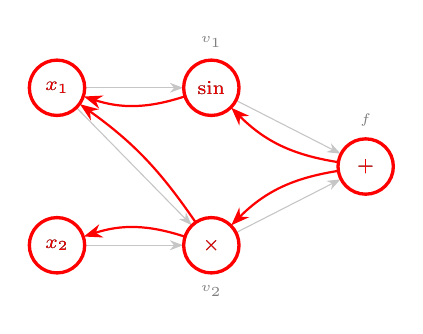
\begin{tikzpicture}[
        x=1.4cm, y=1.0cm, >=Stealth,
        vtx/.style={circle, draw, minimum size=20pt, inner sep=1pt, font=\scriptsize},
        vlab/.style={font=\tiny, gray},
        adj/.style={font=\tiny, red},
        back/.style={->, red, thick}]
        % forward graph (light), drawn first
        \node[vtx] (x1) at (0,1)  {$x_1$};
        \node[vtx] (x2) at (0,-1) {$x_2$};
        \node[vtx] (v1) at (1.4,1)  {$\sin$};
        \node[vtx] (v2) at (1.4,-1) {$\times$};
        \node[vtx] (f)  at (2.8,0)  {$+$};
        \node[vlab, above=1pt of v1] {$v_1$};
        \node[vlab, below=1pt of v2] {$v_2$};
        \node[vlab, above=1pt of f]  {$f$};
        \draw[->, gray!45] (x1) -- (v1);
        \draw[->, gray!45] (x1) -- (v2);
        \draw[->, gray!45] (x2) -- (v2);
        \draw[->, gray!45] (v1) -- (f);
        \draw[->, gray!45] (v2) -- (f);
        % step 1: seed the output adjoint
        \node<2->[vtx, draw=red, very thick, text=red] at (2.8,0) {$+$};
        % \node<2->[adj, right=2pt of f] {$\bar f{=}1$};
        % step 2: adjoints flow back to v1, v2
        \draw<3->[back] (f) to[bend left=18]  (v1);
        \draw<3->[back] (f) to[bend right=18] (v2);
        \node<3->[vtx, draw=red, very thick, text=red] at (1.4,1)  {$\sin$};
        \node<3->[vtx, draw=red, very thick, text=red] at (1.4,-1) {$\times$};
        % step 3: adjoints flow back to the inputs
        \draw<4->[back] (v1) to[bend left=18]  (x1);
        \draw<4->[back] (v2) to[bend right=10] (x1);
        \draw<4->[back] (v2) to[bend right=18] (x2);
        \node<4->[vtx, draw=red, very thick, text=red] at (0,1)  {$x_1$};
        \node<4->[vtx, draw=red, very thick, text=red] at (0,-1) {$x_2$};
      \end{tikzpicture}
    \end{column}
    \begin{column}{0.60\textwidth}
      {\footnotesize
      \textbf{Backward sweep (Chain Rule)} }\\[5pt]
      \uncover<2->{$\bar f = \tfrac{\partial f}{\partial f} = 1$\\[6pt]}
      \uncover<3->{%
        $\bar v_1 = \tfrac{\partial f}{\partial v_1}
          = \tfrac{\partial f}{\partial f}\cdot \tfrac{\partial f}{\partial v_1} = \bar f\cdot 1$\\[3pt]
        $\bar v_2 = \tfrac{\partial f}{\partial v_2}
          = \tfrac{\partial f}{\partial f}\cdot\tfrac{\partial f}{\partial v_2} = \bar f\cdot 1$\\[6pt]}
      \uncover<4->{%
        $\bar x_2 = \tfrac{\partial f}{\partial x_2}
          = \tfrac{\partial f}{\partial v_2}\cdot \tfrac{\partial v_2}{\partial x_2} = \bar v_2\, x_1$\\[3pt]
        $\bar x_1 = \tfrac{\partial f}{\partial x_1}
          = \tfrac{\partial f}{\partial v_1}\cdot \tfrac{\partial v_1}{\partial x_1}
          + \tfrac{\partial f}{\partial v_2}\,\tfrac{\partial v_2}{\partial x_1}$\\[2pt]
        $\hphantom{\bar x_1} = \bar v_1\cos x_1 + \bar v_2\, x_2$}     
    \end{column}
  \end{columns}

  \vfill

  \uncover<5->{
  {\footnotesize One forward pass (store intermediates) $+$ one backward pass. Cost
  $\propto$ \emph{number of outputs} $=1$, \emph{independent of $n$}.}
  }

\end{frame}

\begin{frame}{The cheap-gradient principle}

  \textbf{Theorem (Baur--Strassen, 1983):}
  Computing the gradient $f'(x)\in\Re^n$ costs no more than a small constant
  (in practice $\leq 5$) times the cost of evaluating $f(x)$ itself --- regardless of
  $n$.

  \vfill

  \uncover<2->{
  This is the engine of deep learning:
  \begin{itemize}
    \setlength\itemsep{0.4em}
  \item A gradient over a billion parameters costs about one forward evaluation.
  \item The price is \emph{memory}: the forward pass stores all intermediates for the
    backward pass.
  \end{itemize}
  }


\end{frame}

\section{Adaptive Methods: Momentum and Adam}

\begin{frame}{Why plain SGD struggles}

  \includegraphics[width=0.4\columnwidth]{figures/rosenbrock/rosenbrock.pdf}

  \vfill

  SGD takes the same scalar step $h$ in \emph{every} coordinate
  ($x_{k+1} = x_k - h\, \hat f'(x_k)$), yet deep networks are \emph{wildly}
  ill-conditioned: curvature varies by orders of magnitude across coordinates and across
  the landscape.

  \vfill


  \begin{itemize}
    \setlength\itemsep{0.5em}
  \item A single $h$ is too \emph{large} for steep directions, too \emph{small} for
    flat ones.
  \item Lecture~12's remedy was a \emph{variable metric} $H_k$:
    $x_{k+1} = x_k - H_k^{-1} \hat f'(x_k)$.
  \item<3-> Full $H_k\in\Re^{n\times n}$ is too expensive. \emph{Adam}
    is a practical compromise: a \emph{diagonal}, \emph{running} metric.
  \end{itemize}
  


\end{frame}

\begin{frame}{Momentum (heavy ball)}

  First fix: do not trust a single noisy gradient --- \emph{average} them with an
  exponential moving average ($\beta_1 \approx 0.9$):
  \[
    m_k = \beta_1 m_{k-1} + (1-\beta_1)\, \hat f'(x_k), \qquad
    x_{k+1} = x_k - h\, m_k.
  \]

  \vfill

  \begin{itemize}
    \setlength\itemsep{0.5em}
  \item Averaging helps with noise reduction.
  \item Builds \emph{momentum} along consistent directions, damps oscillation across
    steep valleys.
  \end{itemize}

\end{frame}

\begin{frame}{Per-coordinate step sizes: AdaGrad / RMSProp}

  Second fix: give each coordinate its \emph{own} step size, scaled down where
  gradients have been large. Accumulate a running second moment ($\beta_2\approx0.999$):
  \[
    v_k = \beta_2 v_{k-1} + (1-\beta_2)\, \hat f'(x_k)^{\had 2}
    \qquad (\text{elementwise square}).
  \]

  \vfill

  Then step with a \emph{coordinatewise} learning rate
  \[
    x_{k+1} = x_k - \frac{h}{\sqrt{v_k}+\epsilon}\had \hat f'(x_k).
  \]

  \vfill

  \uncover<2->{
  \begin{itemize}
  \item $\sqrt{v_k}$ estimates the local gradient magnitude per coordinate.
  \item Equivalent to a crude \emph{diagonal} preconditioner $H_k = \diag(\sqrt{v_k}+\epsilon)$.
  \end{itemize}
  }

\end{frame}

\begin{frame}{Adam = Momentum $+$ RMSProp}

  \begin{algorithm}[H]
    \SetKwInput{Initialization}{Initialisation}
    \Initialization{$x_0$, $m_{-1}=0$, $v_{-1}=0$; defaults $\beta_1=0.9,~\beta_2=0.999,~\epsilon=10^{-8}$}
    \For{$k\geq 0$}{
      $g_k \defn \hat f'(x_k)$ \\
      $m_k \defn \beta_1 m_{k-1} + (1-\beta_1) g_k$ \hfill (first moment)\\
      $v_k \defn \beta_2 v_{k-1} + (1-\beta_2) g_k^{\had 2}$ \hfill (second moment)\\
      $\hat m_k \defn m_k/(1-\beta_1^{k+1})$, \quad $\hat v_k \defn v_k/(1-\beta_2^{k+1})$ \hfill (bias correction)\\
      $x_{k+1} \defn x_k - h\, \dfrac{\hat m_k}{\sqrt{\hat v_k}+\epsilon}$
    }
    \caption{Adam (Kingma \& Ba, 2015)}
  \end{algorithm}

  \vfill

  \uncover<2->{
  The bias correction undoes the $m_{-1}=v_{-1}=0$ initialisation: early on
  $\E{}{m_k}\approx(1-\beta_1^{k+1})\E{}{g}$, so we divide it out.
  }

\end{frame}

\begin{frame}{How to read Adam}

  \[
    x_{k+1} = x_k - h\, \underbrace{\frac{1}{\sqrt{\hat v_k}+\epsilon}}_{\text{diagonal metric}} \had \underbrace{\hat m_k}_{\text{smoothed gradient}}
  \]

  \vfill

  \begin{itemize}
    \setlength\itemsep{0.6em}
  \item \emph{Variable metric:} a diagonal approximation to $H_k^{-1}$.
  \item \emph{Per-coordinate scale invariance:} since the step is
    $\hat m_k/\sqrt{\hat v_k}$ \emph{coordinatewise}, rescaling any one coordinate's
    gradient by a constant leaves {its} iterates unchanged.
  \item<2-> \red{Caveat:} on some problems Adam generalises \emph{worse} than plain SGD
    --- a hint that the optimizer shapes the \emph{solution}, not just the speed.
  \end{itemize}

\end{frame}

\section{Generalization: Double Descent and Implicit Regularization}

\begin{frame}{The generalization puzzle}

  \textbf{Optimizers:}
  \[
    \hat x_T \in \arg\min_{x}\E{(\omega,y)\sim \mb D_T}{\ell(h_x(\omega),y)}
  \]

  \vfill

  \textbf{Statisticians:}
  \[
    x^\star \in \arg\min \min_{x}\E{(\omega,y)\sim \mb D}{\ell(h_x(\omega),y)}
  \]

  \vfill

  As the empirical distribution $\mb D_T$ is not the distribution $\mb D$ out-of-sample \emph{overfitting} happens.

  % \vfill

  % \uncover<2->{
  % Modern networks are \emph{overparameterised}: $n \gg T$, more parameters than data.
  % They can \emph{interpolate} --- drive training loss to \emph{zero}, even on randomly
  % relabelled data (Zhang et al., 2017).
  % }

  % \vfill

  % \uncover<3->{
  % Classical statistics screams \emph{overfitting}. Yet these models generalise well.
  % Two facts resolve the paradox: \emph{double descent} and \emph{implicit
  % regularization}.
  % }

\end{frame}

\begin{frame}{Classical wisdom: the bias--variance tradeoff}

  \begin{center}
    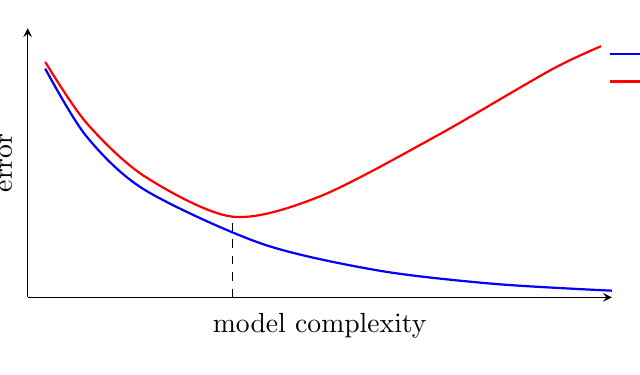
\begin{tikzpicture}[trim axis left, trim axis right]
      \begin{axis}[
        width=9cm, height=5cm,
        axis lines=left, xlabel={model complexity}, ylabel={error},
        xtick=\empty, ytick=\empty, xmin=0, xmax=10, ymin=0, ymax=4,
        legend pos=outer north east,
        legend style={at={(0.98,0.98)}, font=\scriptsize, draw=none}]
        % training error: monotone down
        \addplot[blue, thick, smooth] coordinates {(0.3,3.4)(1,2.4)(2,1.6)(4,0.8)(6,0.4)(8,0.2)(10,0.1)};
        \addlegendentry{training error}
        % test error: U-shape
        \addplot[red, thick, smooth] coordinates {(0.3,3.5)(1,2.6)(2,1.8)(3.5,1.2)(5,1.5)(7,2.4)(9,3.4)(10,3.8)};
        \addlegendentry{test error}
        \draw[dashed] (axis cs:3.5,0) -- (axis cs:3.5,1.2);
        % \node[font=\scriptsize, anchor=south] at (axis cs:3.5,1.25) {sweet spot};
      \end{axis}
    \end{tikzpicture}
  \end{center}

\end{frame}

\begin{frame}{Modern networks are {overparameterised}}

  $n \gg T$, more parameters than data.
  They can \emph{interpolate} --- drive training loss to \emph{zero}, even on randomly
  relabelled data (Zhang et al., 2017).

\end{frame}

\begin{frame}{Double descent}

  \begin{center}
    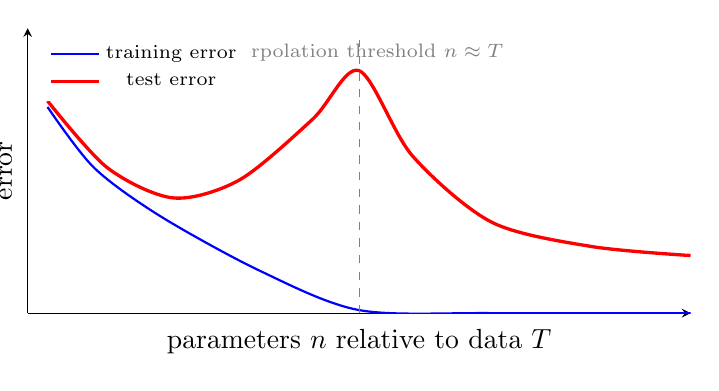
\begin{tikzpicture}[trim axis left, trim axis right]
      \begin{axis}[
        width=10cm, height=5.2cm,
        axis lines=left, xlabel={parameters $n$ relative to data $T$}, ylabel={error},
        xtick=\empty, ytick=\empty, xmin=0, xmax=10, ymin=0, ymax=4.7,
        legend style={at={(0.02,0.98)}, anchor=north west, font=\scriptsize, draw=none}]
        % training error -> 0 past threshold
        \addplot[blue, thick, smooth] coordinates {(0.3,3.4)(1,2.4)(2,1.6)(3.5,0.7)(5,0.05)(7,0)(10,0)};
        \addlegendentry{training error}
        % test error: classical U then a second descent past the threshold
        \addplot[red, very thick, smooth] coordinates {(0.3,3.5)(1.2,2.4)(2.2,1.9)(3.2,2.2)(4.3,3.2)(5,4.0)(5.8,2.6)(7,1.5)(8.5,1.1)(10,0.95)};
        \addlegendentry{test error}
        \draw[dashed, gray] (axis cs:5,0) -- (axis cs:5,4.5);
        \node[font=\scriptsize, anchor=south, gray] at (axis cs:5,4) {interpolation threshold $n\approx T$};
        % \node[font=\scriptsize, anchor=north, gray] at (axis cs:2.6,1.5) {classical};
        % \node[font=\scriptsize, anchor=north, gray] at (axis cs:8.0,2.4) {modern};
      \end{axis}
    \end{tikzpicture}
  \end{center}

  \vfill

  \emph{Belkin, Hsu, Ma \& Mandal (2019):} the classical U-curve is only half the story.
  Push \emph{past} the interpolation threshold and the test error \emph{descends again} ---
  bigger models generalise \emph{better}!?

\end{frame}

\begin{frame}{Double descent --- what is going on?}

  \textbf{ERM:}
  \[
    \hat x_T \in \arg\min_{x}\E{(\omega,y)\sim \mb D_T}{\ell(h_x(\omega),y)}
  \]

  \vfill
  
  \begin{center}
    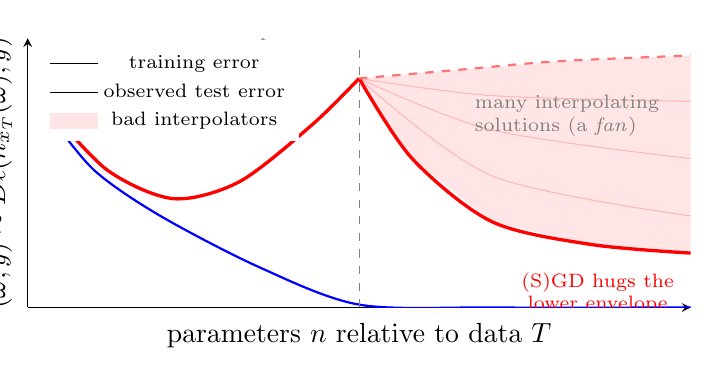
\begin{tikzpicture}[trim axis left, trim axis right]
      \begin{axis}[
        width=10cm, height=5.0cm,
        axis lines=left, xlabel={parameters $n$ relative to data $T$}, ylabel={$\E{(\omega,y)\sim \mb D}{\ell(h_{\hat x_T}(\omega),y)}$},
        xtick=\empty, ytick=\empty, xmin=0, xmax=10, ymin=0, ymax=4.7,
        legend style={at={(0.02,0.98)}, anchor=north west, font=\scriptsize, draw=none}]

        % ----- fan of interpolating solutions (past the threshold) -----
        \addplot[draw=none, name path=fanhi] coordinates {(5,4.0)(6.5,4.15)(8,4.3)(10,4.4)};
        \addplot[draw=none, name path=fanlo] coordinates {(5,4.0)(5.8,2.6)(7,1.5)(8.5,1.1)(10,0.95)};
        \addplot[red!10] fill between[of=fanhi and fanlo];
        % a few representative interpolating solutions inside the fan
        \addplot[red!28, thin, smooth] coordinates {(5,4.0)(7,3.7)(10,3.6)};
        \addplot[red!28, thin, smooth] coordinates {(5,4.0)(7,3.1)(10,2.6)};
        \addplot[red!28, thin, smooth] coordinates {(5,4.0)(7,2.3)(10,1.6)};

        % ----- training error -> 0 past threshold -----
        \addplot[blue, thick, smooth] coordinates {(0.3,3.4)(1,2.4)(2,1.6)(3.5,0.7)(5,0.05)(7,0)(10,0)};
        \addlegendentry{training error}

        % ----- observed test error: classical branch + the lower envelope -----
        \addplot[red, very thick, smooth] coordinates {(0.3,3.5)(1.2,2.4)(2.2,1.9)(3.2,2.2)(4.3,3.2)(5,4.0)};
        \addlegendentry{observed test error}
        \addplot[red, very thick, smooth] coordinates {(5,4.0)(5.8,2.6)(7,1.5)(8.5,1.1)(10,0.95)};
        % upper envelope: the bad interpolators
        \addplot[red!55, thick, dashed, smooth] coordinates {(5,4.0)(6.5,4.15)(8,4.3)(10,4.4)};
        \addlegendentry{bad interpolators}

        % threshold + annotations
        \draw[dashed, gray] (axis cs:5,0) -- (axis cs:5,4.5);
        \node[font=\scriptsize, anchor=south, gray] at (axis cs:5,4.5) {interpolation threshold $n\approx T$};
        \node[font=\scriptsize, anchor=west, gray, align=left] at (axis cs:6.6,3.35)
          {many interpolating\\ solutions (a \emph{fan})};
        \node[font=\scriptsize, anchor=north, red, align=center] at (axis cs:8.6,0.78)
          {(S)GD hugs the\\ lower envelope};
      \end{axis}
    \end{tikzpicture}
  \end{center}

\end{frame}

\begin{frame}{Implicit bias, provably: least squares}

  \textbf{Theorem:} Let $f(x)=\tfrac12\norm{Ax-y}^2$ with $A\in\Re^{T\times n}$,
  $n>T$, $A$ full row rank (so infinitely many interpolants exist). Gradient descent
  (or SGD) started at $x_0=0$ converges to the \emph{minimum-norm} interpolant
  \[
    x^\star = \arg\min\big\{ \norm{x}_2 ~:~ Ax = y \big\} = A\tpose (A A\tpose)^{-1} y.
  \]

  \vfill

  \textbf{Proof:} Each step $x_{k+1}=x_k - h A\tpose(Ax_k-y)$ adds a vector in
  $\mr{row}(A)=\mr{range}(A\tpose)$. Hence every iterate lies in $x_0 + \mr{row}(A) = \mr{row}(A)$.
  The interpolation set $\{x:Ax=y\}$ meets the subspace $\mr{row}(A)$ in exactly one
  point --- the minimum-norm solution --- and that is where the iterates converge.
  \hfill$\square$

\end{frame}

\begin{frame}{Flat versus sharp minima}

  A complementary geometric view: not all zero-loss minima are equal.

  \vfill

  \begin{center}
    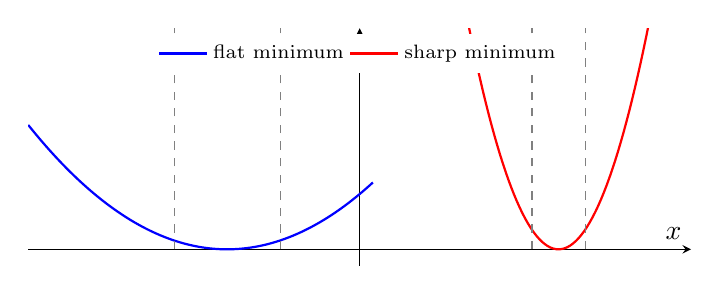
\begin{tikzpicture}
      \begin{axis}[
        width=10cm, height=4.6cm,
        axis lines=middle, xlabel={$x$}, ylabel={loss},
        xtick=\empty, ytick=\empty, xmin=-5, xmax=5, ymin=-0.3, ymax=4,
        domain=-5:5, samples=100,
        legend style={at={(0.5,0.98)}, anchor=north, font=\scriptsize, draw=none, legend columns=2}]
        \addplot[blue, thick, domain=-5:0.2] {0.25*(x+2)^2};   \addlegendentry{flat minimum}
        \addplot[red, thick, domain=0.8:5] {2.2*(x-3)^2};       \addlegendentry{sharp minimum}
        % perturbation bands
        \draw[dashed, gray] (axis cs:-2.8,0) -- (axis cs:-2.8,4);
        \draw[dashed, gray] (axis cs:-1.2,0) -- (axis cs:-1.2,4);
        \draw[dashed, gray] (axis cs:2.6,0) -- (axis cs:2.6,4);
        \draw[dashed, gray] (axis cs:3.4,0) -- (axis cs:3.4,4);
      \end{axis}
    \end{tikzpicture}
  \end{center}

\end{frame}

\begin{frame}{Sharp minima are unstable [$\star$]}

  \textbf{Theorem:} for $\Phi(x) = x - h\, f'(x)$ with $H=\nabla^2 f(x^\star)\succeq 0$, the
  minimum $x^\star$ is a \emph{linearly stable} fixed point iff
  $\lambda_{\max}(H)\leq 2/h$. \quad (\emph{same $\frac{2}{L}$ story as Lecture~8})

  \vfill

  \begin{center}
    \begin{minipage}{0.46\textwidth}\centering
      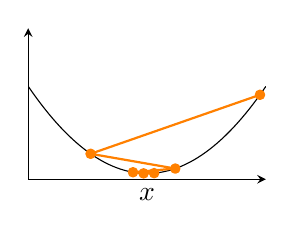
\begin{tikzpicture}
        \begin{axis}[width=4.6cm, height=3.5cm, axis lines=left, ticks=none,
          xlabel={$x$}, clip=true, xmin=-2, xmax=2, ymin=-0.2, ymax=5]
          \addplot[black, samples=60, domain=-2:2] {0.75*x^2};
          \addplot[orange, thick, line join=round, mark=*, mark size=1.5pt]
            coordinates {(1.900,2.708)(-0.950,0.677)(0.475,0.169)(-0.237,0.042)(0.119,0.011)(-0.059,0.003)};
        \end{axis}
      \end{tikzpicture}\\[0.2em]
      {\scriptsize \green{flat}: $\lambda=1.5<\tfrac{2}{h}$ --- \green{converges}}
    \end{minipage}\hfill
    \begin{minipage}{0.46\textwidth}\centering
      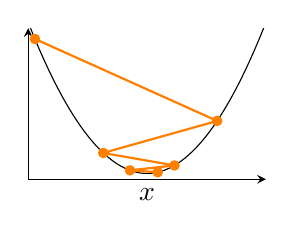
\begin{tikzpicture}
        \begin{axis}[width=4.6cm, height=3.5cm, axis lines=left, ticks=none,
          xlabel={$x$}, clip=true, xmin=-2, xmax=2, ymin=-0.2, ymax=5]
          \addplot[black, samples=60, domain=-2:2] {1.3*x^2};
          \addplot[orange, thick, line join=round, mark=*, mark size=1.5pt]
            coordinates {(0.180,0.042)(-0.288,0.108)(0.461,0.276)(-0.737,0.707)(1.180,1.809)(-1.887,4.631)};
        \end{axis}
      \end{tikzpicture}\\[0.2em]
      {\scriptsize \red{sharp}: $\lambda=2.6>\tfrac{2}{h}$ --- \red{diverges}}
    \end{minipage}
  \end{center}

  \vfill

  \textbf{Why:} near $x^\star$, $e_k = x_k-x^\star$ obeys $e_{k+1}=(I-hH)e_k$; along an
  eigendirection $e_{k+1}=(1-h\lambda)e_k$, which contracts iff $|1-h\lambda|\leq1$, i.e.\
  $\lambda\leq 2/h$. A \emph{sharp} minimum (large $\lambda$) is \emph{repelling}, so (S)GD
  is pushed toward \emph{flat} ones --- implicit regularisation.

\end{frame}

\end{document}
%%% Local Variables:
%%% mode: latex
%%% TeX-master: t
%%% End:
